%% This is file `elsarticle-template-1-num.tex',
%%
%% Copyright 2009 Elsevier Ltd
%%
%% This file is part of the 'Elsarticle Bundle'.
%% ---------------------------------------------
%%
%% It may be distributed under the conditions of the LaTeX Project Public
%% License, either version 1.2 of this license or (at your option) any
%% later version.  The latest version of this license is in
%%    http://www.latex-project.org/lppl.txt
%% and version 1.2 or later is part of all distributions of LaTeX
%% version 1999/12/01 or later.
%%
%% The list of all files belonging to the 'Elsarticle Bundle' is
%% given in the file `manifest.txt'.
%%
%% Template article for Elsevier's document class `elsarticle'
%% with numbered style bibliographic references
%%
%% $Id: elsarticle-template-1-num.tex 149 2009-10-08 05:01:15Z rishi $
%% $URL: http://lenova.river-valley.com/svn/elsbst/trunk/elsarticle-template-1-num.tex $
%%
\documentclass[preprint,review,12pt]{elsarticle}

%% Use the option review to obtain double line spacing
%% \documentclass[preprint,review,12pt]{elsarticle}

%% Use the options 1p,twocolumn; 3p; 3p,twocolumn; 5p; or 5p,twocolumn
%% for a journal layout:
%% \documentclass[final,1p,times]{elsarticle}
%% \documentclass[final,1p,times,twocolumn]{elsarticle}
%% \documentclass[final,3p,times]{elsarticle}
%% \documentclass[final,3p,times,twocolumn]{elsarticle}
%% \documentclass[final,5p,times]{elsarticle}
%% \documentclass[final,5p,times,twocolumn]{elsarticle}

%% if you use PostScript figures in your article
%% use the graphics package for simple commands
\usepackage{graphics}
%% or use the graphicx package for more complicated commands
\usepackage{graphicx}
%% or use the epsfig package if you prefer to use the old commands
\usepackage{epsfig}
\usepackage{epstopdf}
%% The amssymb package provides various useful mathematical symbols
\usepackage{amssymb}
%% The amsthm package provides extended theorem environments
%% \usepackage{amsthm}

%% The lineno packages adds line numbers. Start line numbering with
%% \begin{linenumbers}, end it with \end{linenumbers}. Or switch it on
%% for the whole article with \linenumbers after \end{frontmatter}.
%% \usepackage{lineno}

%% natbib.sty is loaded by default. However, natbib options can be
%% provided with \biboptions{...} command. Following options are
%% valid:

%%   round  -  round parentheses are used (default)
%%   square -  square brackets are used   [option]
%%   curly  -  curly braces are used      {option}
%%   angle  -  angle brackets are used    <option>
%%   semicolon  -  multiple citations separated by semi-colon
%%   colon  - same as semicolon, an earlier confusion
%%   comma  -  separated by comma
%%   numbers-  selects numerical citations
%%   super  -  numerical citations as superscripts
%%   sort   -  sorts multiple citations according to order in ref. list
%%   sort&compress   -  like sort, but also compresses numerical citations
%%   compress - compresses without sorting
%%
%% \biboptions{comma,round}

% \biboptions{}
\usepackage{color,url,amsmath}

\newcommand\fxbox[1]{\center{\framebox[1.1\width][c]{\strut#1}}}
\newcommand\mxbox[1]{\center{\makebox[1.1\width][c]{\strut#1}}}


\journal{Knowledge Based Systems}

\begin{document}

\begin{frontmatter}

%% Title, authors and addresses

%% use the tnoteref command within \title for footnotes
%% use the tnotetext command for the associated footnote;
%% use the fnref command within \author or \address for footnotes;
%% use the fntext command for the associated footnote;
%% use the corref command within \author for corresponding author footnotes;
%% use the cortext command for the associated footnote;
%% use the ead command for the email address,
%% and the form \ead[url] for the home page:
%%
%% \title{Title\tnoteref{label1}}
%% \tnotetext[label1]{}
%% \author{Name\corref{cor1}\fnref{label2}}
%% \ead{email address}
%% \ead[url]{home page}
%% \fntext[label2]{}
%% \cortext[cor1]{}
%% \address{Address\fnref{label3}}
%% \fntext[label3]{}

\title{A Graph Based Approach for Contextual Text Normalization}

%% use optional labels to link authors explicitly to addresses:
%% \author[label1,label2]{<author name>}
%% \address[label1]{<address>}
%% \address[label2]{<address>}

\author{}

\address{}

\begin{abstract}
%% Text of abstract
%The huge amount of data available in social media provide interesting opportunities for several text analytics applications such as sentiment analysis and event detection.

The informal nature of social media text render is very difficult to be automatically processed by natural language processing tools. Text normalization, which corresponds to restoring the noisy words to their canonical forms, provides a solution to this challenge.
We introduce an unsupervised text normalization approach that utilizes not only lexical, but also contextual and grammatical features of social text.
The contextual and grammatical features are extracted from a word association graph built by using a large unlabeled social media text corpus.
The graph encodes the relative positions of the words with respect to each other, as well as their part-of-speech tags.
The lexical features are obtained by using the longest common subsequence ratio and edit distance measures to encode the surface similarity among words, and the double metaphone algorithm to represent the phonetic similarity. Unlike most of the recent approaches that are based on generating normalization dictionaries, the proposed approach performs normalization by considering the context of the noisy words in the input text.
%In other words, a noisy word can be normalized to different canonical forms depending on the context of the word in the input text message.
Our results show that it achieves state-of-the-art F-score performance on a standard data set. In addition, the system can be tuned to achieve very high precision without sacrificing much from recall.

\end{abstract}

\begin{keyword}
%% keywords here, in the form: keyword \sep keyword
Text Normalization \sep Twitter \sep micro-blogs \sep social media
%% MSC codes here, in the form: \MSC code \sep code
%% or \MSC[2008] code \sep code (2000 is the default)

\end{keyword}

\end{frontmatter}

%%
%% Start line numbering here if you want
%%
% \linenumbers

%% main text

\section{Introduction}
\label{sec:introduction}

Within the last decade, the common belief among internet users, that social text has (or should have) it's own lexical and grammatical features, has naturally given birth to an internet language and jargon; which has been steadily growing and evolving ever since ~\cite{Choudhury:2007:IMS:1326044.1326048, eisenstein2013bad}. This behavioral preference phenomenon brings another challenge of its own. Not only is the internet jargon itself growing and evolving in an exponential pace, but also since the beginning of World Wide Web, internet has it's own slang. \textit{lol} meaning \textit{laughing out loudly},  \textit{xoxo} meaning \textit{kissing}, \textit{4u} meaning \textit{for you} are the among the most commonly used examples of this slang. In addition, these specific forms of informal expressions in social text usually take many different lexical forms when generated by each individual; even though the intended contextual meaning might be the same~\cite{eisenstein2013bad}. In other words, with each different individual the same content is being expressed (written) in different ways. Due to this unpredicted variety of such expressions, it would be appropriate to call this divergency "noise" in social text.

The scope of the problem doesn't end there. In addition, within the last few years, by the increasing use of mobile devices, social text has now been preferred to be transcribed by using Speech-to-Text (STT) tools. This text input preference is getting trendier and being used more frequently. The insufficient accuracy of such STT tools brings considerable amount of ``additional noise'' to social text. Tools such as spellcheckers and slang dictionaries have proven to be insufficient to cope with this challenge long time ago~\cite{sproat2001normalization}.

Lastly, when we also consider the usual scarcity of attention when people post messages on social media platforms, the problem of analyzing social text actually goes beyond the reach of human cognitive capacity. The mass usage of such social media platforms, makes it impossible to derive analysis results in a limited time scope when processed manually. In addition, most automatic Natural Language Processing (NLP) tools such as named entity recognizers and  dependency parsers generally perform poorly on social media text~\cite{ritter2010unsupervised}.

Text normalization is a preprocessing step to restore noisy words in text to their original (canonical) forms~\cite{Han:2011:LNS:2002472.2002520} to make use in NLP applications or more broadly to understand the digitized text better. For example, \textit{talk 2 u later} can be normalized as \textit{talk to you later} or similarly \textit{enormoooos, enrmss, enourmos} can be normalized as \textit{enormous}. These noisy tokens are referred as Out of Vocabulary (OOV) words. The normalization task restores the OOV words to their In Vocabulary~(IV) forms. Table \ref{tab:normalizations} shows sample OOV words encountered in social media text and their corresponding IV forms.

\begin{table}[tbhp]
\begin{minipage}[c]{.5\linewidth}
\centering
\begin{tabular}[h]{|r|r|}
\hline
ppl & people \\
havent & haven't \\
tmr &   tomorrow \\
soooo &  so \\
sooon &  soon \\
raight & right \\
raight & alright \\
\hline
\end{tabular}
\end{minipage}
\begin{minipage}[c]{.5\linewidth}
\centering
\begin{tabular}[h]{|r|r|}
\hline
r  &  are \\
mor &    more \\
doin &   doing \\
n &      and \\
friiied &  fried \\
finge &  finger \\
kissin & kissing \\
\hline
\end{tabular}
\end{minipage}
\caption{Sample noisy tokens and their normalized forms.}
\label{tab:normalizations}
\end{table}

Every OOV word should not be considered for normalization. The social text is continuously evolving with new words and named entities that are not in the vocabularies of the systems~\cite{DBLP:conf/acl/HassanM13}. The OOV tokens that should be considered for normalization are referred to as ill-formed words. Oppositely an OOV word can sometimes lexically fit an IV word (Ex:~\textit{tanks} is both an IV word and an OOV word with the canonical form \textit{thanks}).
%The task of recognizing which tokens are OOV, and which of those are ill-formed are beyond the scope of this paper.

In~\cite{Choudhury:2007:IMS:1326044.1326048} Choudhury et Al.~proposes that the OOV words observed in noisy text can be classified into two groups, unintentional and intentional errors. The unintentional errors are caused by (1) pressing of the wrong key, (2) pressing of a key more than the desired number of times, (3) deletion of a character or (4) inadequate knowledge of spelling. As for the intentional errors, they can be categorized into four categories: character deletion(``tlk'' for ``talk'', ``msg'' for ``message'', ``tomoro'' for ``tomorrow'', ``mob'' for ``mobile''), phonetic substitution~(``nite'' for ``night'', ``bk'' for ``back'', ``u'' for ``you'', ``m8'' for ``mate''), abbreviations~(``btw'' for ``by the way'', ``kgp'' for ``Kharagpur'') and non-standard usage~(``wanna'' for ``want to'', ``betta'' for ``better'', ``sumfin'' for ``something'', ``b/c'' for ``because'').

In this paper, we propose a graph based text normalization method that utilizes both contextual and grammatical features of social text. The contextual information of words is modeled by a word association graph that is created from a large social media text corpus. The graph represents the relative positions of the words in the social media text messages and their Part-of-Speech (POS) tags. The lexical similarity features among the words are modeled using the longest common subsequence ratio and edit distance that encode the surface similarity and the double metaphone algorithm that encodes the phonetic similarity. The proposed approach is unsupervised, which is an important advantage over supervised systems, given the continuously evolving language in the social media domain. The same OOV word may have different appropriate normalizations depending on the context of the input text message. Recently proposed dictionary-based text normalization systems perform dictionary look-up and always normalize the same OOV word to the same IV word regardless of the context of the input text ~\cite{Han:2011:LNS:2002472.2002520,DBLP:conf/acl/HassanM13}. On the other hand, the proposed approach does not only make use of the general context information in a large corpus of social media text, but it also makes use of the context of the OOV word in the input text message. Thus, an OOV word can be normalized to different IV words depending on the context of the input text. Another strength of the proposed system is that it achieves the state-of-the art precision scores, without sacrificing from recall.

\section{Related Work}
\label{sec:related}

Early work on text normalization mostly made use of noisy channel model. The first work that had a significant performance improvement over the previous research was Brill and Moore,2000~\cite{Brill:2000:IEM:1075218.1075255}. They proposed a novel noisy channel model for spell checking based on string to string edits. Their error model depended on probabilistic modelling of sub-string transformations. Toutanova et al.,2002 improved this approach by extending the error model with phonetic similarities over words~\cite{Toutanova:2002:PMI:1073083.1073109}.

Choudhury et al.,2007 developed a supervised Hidden Markov Model based approach for normalizing SMS Texts~\cite{Choudhury:2007:IMS:1326044.1326048}. Cook and Stevenson,2009 has expanded this model by introducing an unsupervised noisy channel model~\cite{Cook:2009:UMT:1642011.1642021}. Rather than using one generic model for all word formations as in Choudhury et al.,2007, they used a mixture model in which each different word formation type was modelled explicitly. Aw et al.,2006 proposed a phrase-based statistical MT model for the task~\cite{Aw:2006:PSM:1273073.1273078}. They defined the problem as translating the SMS language to English language.

The down side of these methods were: (1) they did not consider contextual features and (2) each of them observed that tokens have unique normalization. However, that is not the case for the normalization task. The OOV tokens are ambiguous and without contextual information it is not possible to build models that can disambiguate transformations correctly.

Also the supervised models were required annotated data, which is not available for normalized text~\cite{DBLP:conf/wsdm/YangL11} and difficult to create.

More recent approaches handled the text normalization task by building normalization lexicons. Han et al.,2011 developed a two phased model where they only consider the OOV words for normalization~\cite{Han:2011:LNS:2002472.2002520}. First a confusion set is generated using the lexical and phonetic distance features. Latter the candidates in the confusion set is ranked using a mixture of dictionary lookup, word similarity based on lexical edit distance, phonemic edit distance, prefix sub-string, suffix sub-string and longest common subsequence(LCS) and context support metrics.

Gouws et al.,2011 on the other hand, proposed an approach that depended highly on contextual information such as the geological location of the users and twitter client that the tweet is received from~\cite{Gouws:2011:CBL:2021109.2021113}. Using contextual metrics they modelled the transformation distributions.

Liu et al.,2012 proposed a broad coverage normalization system integrates an extended noisy channel model, that is based on enhanced letter transformations, visual priming, string and phonetic similarity~\cite{liu2012broad}. They try to improve the performance of top n normalization candidates by integrating human perspective modeling.

Hassan and Menezes,2013 generated a normalization equivalences lexicon using Markov random walks on a contextual similarity lattice~\cite{DBLP:conf/acl/HassanM13}. One of the biggest difference between our systems are they make use a huge clean vocabulary.

Most recent work on text normalization is the unsupervised log linear model of Yang and Eisenstein,2013~\cite{DBLP:conf/wsdm/YangL11}. Their joint statistical approach uses local context based on an LM and surface similarity.

Along with dictionary based models, Yang and Eisenstein's model have obtained a significant improvement on the performance of text normalization systems. We believe several models such as the morphophonemic similarity, MT, Maximum Likelihood, etc. has their own limits. Higher performance text normalization systems should make use of contextual analysis.



\section{Methodology}
\label{sec:method}

%Unsupervised and graph based context aware model:

%In our model we made use of both lexical, contextual and shallow properties of the noisy text which makes use of a weighted token co-occurrence graph.

In this paper, we propose a graph based approach that models both contextual and lexical similarity features among an OOV word that requires normalization and candidate IV words. A high level overview of our system is shown in Figure~\ref{fig:overview}. An input text is first preprocessed by tokenizing and Part-Of-Speech (POS) tagging. If the text contains an OOV word, the normalization candidates are chosen by making use of the contextual features which are extracted from a pre-generated directed word association graph, as well as lexical similarity features. Lexical similarity features are based on edit distance, longest common subsequence ratio, and double metaphone distance. In addition, a slang dictionary is used as an external resource to enrich the normalization candidate set. The details of the approach are explained in the following sub-sections.

%%% FIGURE
\begin{figure}[htb]
\begin{center}
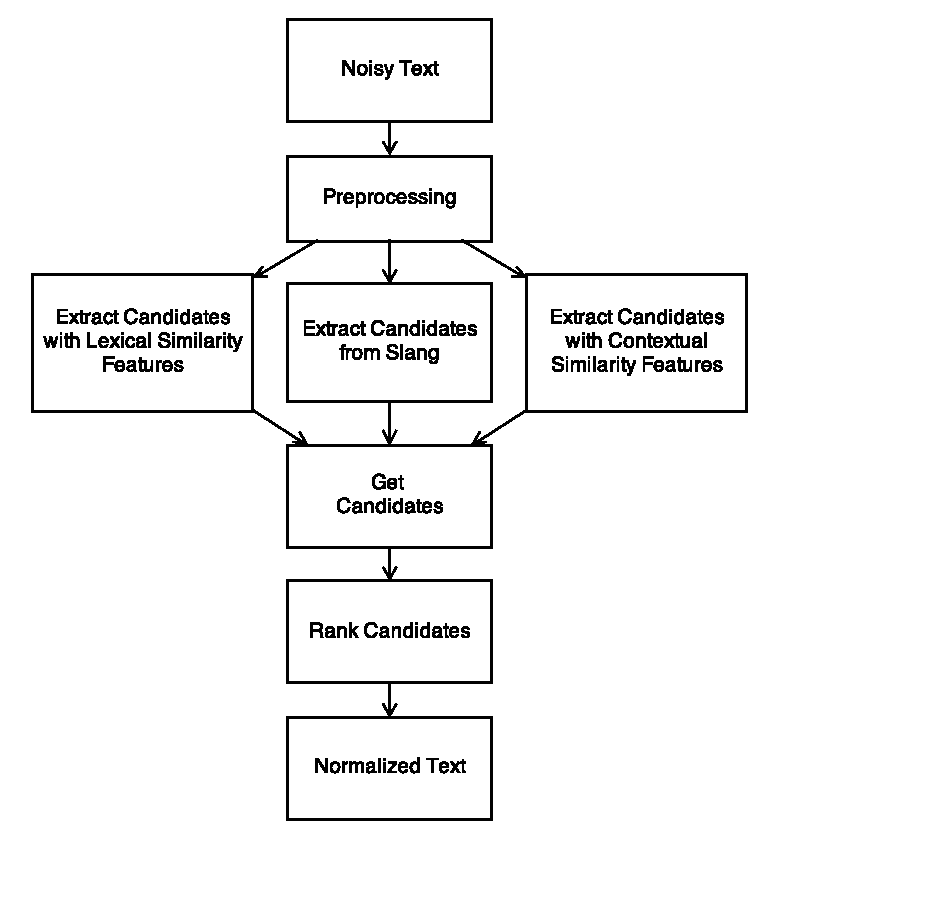
\includegraphics[scale=0.6]{fig/overview}
\caption{High level overview of our system}
\label{fig:overview}
\end{center}
\end{figure}

\subsection{Preprocessing}

%Tokenization is the first step in our system. Tokenization is the process of breaking the text into words, numbers, symbols, emoticons After tokenization, next in the pipeline is POS tagging each token using a social media POS tagger. Unlike the normal POS taggers, social media POS taggers~\cite{DBLP:conf/naacl/OwoputiODGSS13}\cite{Gimpel:2011:PTT:2002736.2002747} provide a broader set of tags that is special to the social text. By this extended set of tags we can identify tokens such as discourse markers~(rt for retweets, cont. for a tweet whose content follows up in the coming tweet) or URLs. So that we can process those tokens within their context.

Tokenization is the first step in our system. It is the process of breaking the text into tokens, which are the smallest meaningful elements such as numbers, symbols, and emoticons. After tokenization, the next step in the pipeline is Part-of-Speech (POS) tagging each token using a POS tagger specifically designed for social media text. Unlike the regular POS taggers designed for well-written newswire-like text, social media POS taggers provide a broader set of tags specific to the peculiarities of social text ~\cite{DBLP:conf/naacl/OwoputiODGSS13,Gimpel:2011:PTT:2002736.2002747}. Using this extended set of tags we can identify tokens such as discourse markers~(e.g. rt for retweets, cont. for a tweet whose content follows up in the coming tweet) or URLs. This enables us to better model the context of the words in social media text.

As shown in Table~\ref{tab:postags}, after preprocessing, each token is assigned a POS tag with a confidence measure between 0 and 1. Later, we use these confidence scores in calculating the edge weights in our context graph. Note that even though the words \emph{w} and\emph{ beatiful} are misspelled, they are tagged correctly by the tagger, with lower confidence scores though.

\begin{table}[htbp]
\begin{minipage}{.5\linewidth}
\begin{tabular}[h]{|llr|}
 \hline
Token & POS tag & Confidence \\
 \hline
with & P & 0.9963 \\
 \hline
a & D & 0.998 \\
 \hline
beautiful & A & 0.9971 \\
 \hline
smile & N & 0.9712 \\
 \hline
\end{tabular}
\end{minipage}
\begin{minipage}{.5\linewidth}
\begin{tabular}[h]{|llr|}
 \hline
Token & POS tag & Confidence \\
 \hline
w & P & 0.7486 \\
 \hline
a & D & 0.9920 \\
 \hline
beatiful & A & 0.9733 \\
 \hline
smile & N & 0.9806 \\
 \hline
\end{tabular}
\end{minipage}
\caption{Sample POS tagger output obtained by using CMU Ark Tagger (P:Pronoun, D:Determiner, A:Adjective, N:Noun, G:Miscellaneous)~\cite{DBLP:conf/naacl/OwoputiODGSS13,Gimpel:2011:PTT:2002736.2002747}}
\label{tab:postags}
\end{table}

\subsection{Graph construction}

Contextual information of words is modeled through a word association graph created by using a large corpus of social media text. The graph encodes the relative positions of the POS tagged words in the text with respect to each other. After preprocessing, each text message in the corpus is traversed in order to extract the nodes and the edges of the graph.
%The graph~(See Figure~\ref{fig:graph}) is build using a big dataset of social media text. After preprocessing, we traverse each entry in the dataset and extract nodes and edges.
A node is defined with four properties: \textit{id, oov, freq, tag}. The token itself and it's POS tag form the \textit{id} field. The \textit{freq} property indicates the node's frequency count in the dataset. The \textit{oov} field is set to True if the token is an OOV word. Following the prior work by Han and Baldwin, 2011 we used the GNU Aspell dictionary (v0.60.6) to determine whether a word is OOV or not~\cite{Han:2011:LNS:2002472.2002520}. Table~\ref{tab:graph} shows a sample tokenized and tagged sentence from the corpus, as well as the nodes and edges that are extracted from it to create the word association graph. A portion of the graph that covers this sample sentence is shown in Figure~\ref{fig:graph}.

\begin{table}[tbhp]
\begin{minipage}[c]{\linewidth}
\fxbox{
Let's$_{\textcolor{red}{L}}$ start$_{\textcolor{red}V}$ this$_{\textcolor{red}D}$ morning$_{\textcolor{red}N}$ w$_{\textcolor{red}P}$ a$_{\textcolor{red}D}$ beatiful$_{\textcolor{red}A}$ smile$_{\textcolor{red}N}$.$_{\textcolor{red},}$
 }\par
\vspace{5mm}
\end{minipage}
\begin{minipage}[c]{\linewidth}
\begin{tabular}[h]{l|l}
Tokens & Let's, start, this, morning, w, a, beatiful, smile,~. \\
\hline
Nodes & Let's$|$L, start$|$V, this$|$D, morning$|$N, w$|$P, a$|$D, beatiful$|$A, smile$|$N, .$|$, \\
\hline
Edges & \{Let's$|$L, start$|$V , distance:1\},\{Let's$|$L, this$|$D, distance:2\}, \\
& ... \\
& \{a$|$D, beatiful$|$A, distance:1\}, \{a$|$D, smile$|$N, distance:2\}, \\
& \{beatiful$|$A, smile$|$N, distance:1\} \\
\end{tabular}
\end{minipage}
\caption{Sample tokenized, POS tagged sentence and the corresponding nodes and edges in the word association graph.}
\label{tab:graph}
\end{table}

\begin{figure}[htb]
\begin{center}
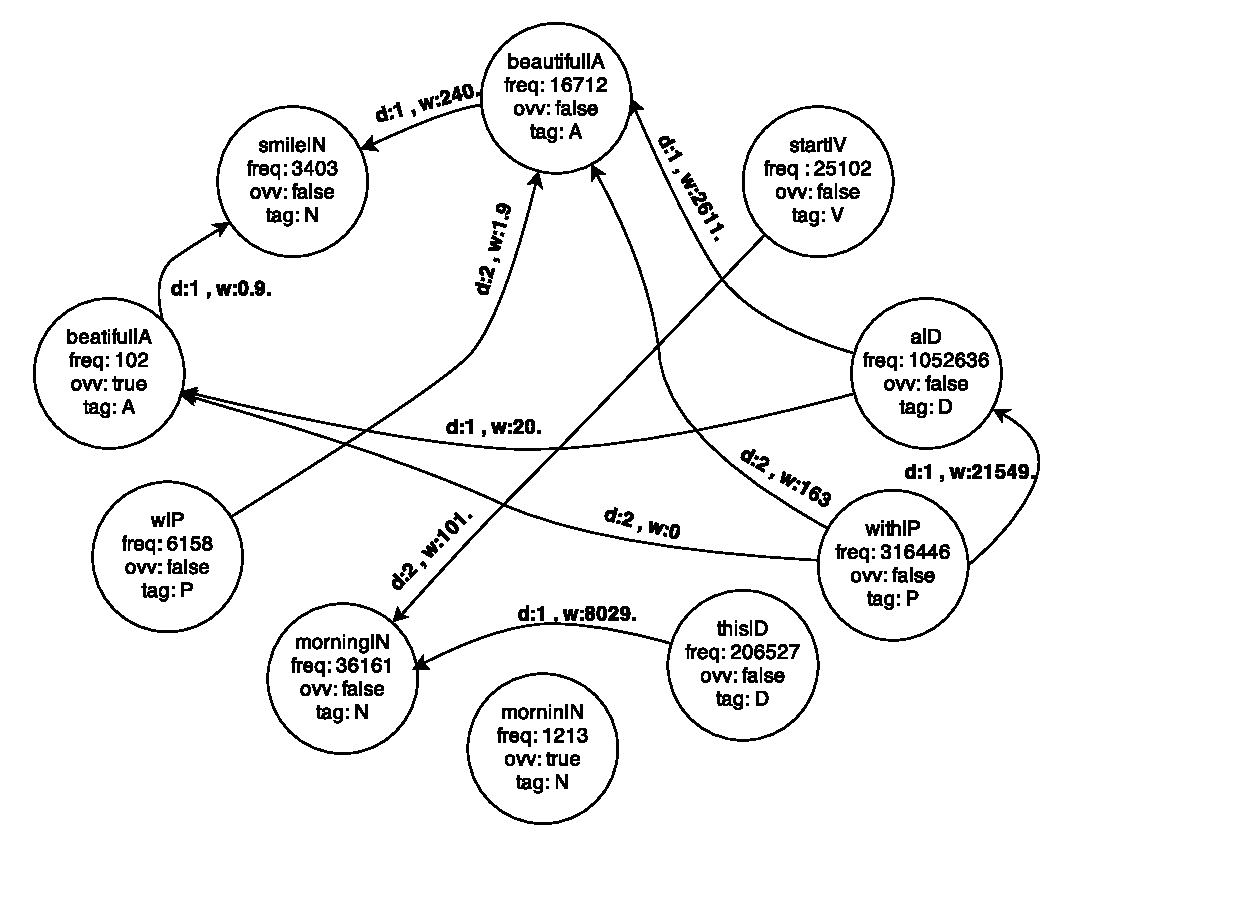
\includegraphics[scale=0.6]{fig/graph}
\caption{Sample nodes and edges from the word association graph.}
\label{fig:graph}
\end{center}
\end{figure}

%We define a node with four properties \textit{id, oov, freq, tag}. The token itself plus it's POS tag forms the \textit{id} field. \textit{freq} property indicates the node's frequency count in the dataset. \textit{oov} field is set to True if the token is a OOV word. Following ~\cite{Han:2011:LNS:2002472.2002520} we used GNU Aspell dictionary (v0.60.6) to determine whether a word is OOV or not.

%In the word-relatedness graph, each node is a unique set of a token and a POS tag (see Table~\ref{tab:graph}). This helps us to identify the tokens not only lexically and contextually but also (in terms of POS tags) grammatically.

In the created word association graph, each node is a unique set of a token and its POS tag. This helps us to identify the candidate IV words for a given OOV word by considering not only lexical and contextual similarity, but also grammatical similarity in terms of POS tags. For example if the token \textit{smile} has been frequently seen as a Noun or a Verb, and not in other forms in the dataset~(e.g.~Table~\ref{tab:nodes}), this provides evidence that it is not a good IV candidate as a normalization for an OOV token that has  been tagged as a Pronoun. On the other hand, \textit{smile} can be a good candidate for a Noun or a Verb OOV token, if it is lexically and contextually similar to it.

\begin{table}[hbt]
  \centering
  \begin{tabular}[tc]{l}
    node id : smile$|$A , freq : 3, oov : False, tag : A \\
    node id : smile$|$N , freq : 3403, oov : False, tag : N \\
    node id : smile$|$V , freq : 2796, oov : False, tag : V \\
  \end{tabular}
  \caption{The nodes in the word association graph representing the token \textit{smile} tagged with different POS tags.}
\label{tab:nodes}
\end{table}

An edge is created between two nodes in the graph, if the corresponding word pair (i.e. token/POS pair) are contextually associated. Two words are considered as contextually associated if they satisfy the following criteria:

\begin{itemize}
\item The two words co-occur within a maximum word distance of $d_t$ in a text message in the corpus.
\item Each word has a minimum frequency of $f_t$ in the corpus.
\end{itemize}

The directionality of the edges is based  on the sequence of words in the text messages in the corpus. In other words, an edge between two nodes is directed from the earlier seen token towards the later seen token. For example, Table~\ref{tab:edges} shows the edges that would be derived from a text including the phrase ``with a beautiful smile''. The \textit{from} property indicates the first word and \textit{to} is the latter in the phrase. The direction and the distance together represent a unique triplet. For each pair of nodes with a specific distance there is an edge with a positive weight, if the two nodes are related. Each co-occurrence of two related nodes increases the weight of the edge between them with an average of the nodes' POS tag confidence scores in the text message considered. If we are to expand the graph with the example phrase shown in Table~\ref{tab:edges}, the weight of the edge with distance $3$ from the node \emph{with$|$P}  to the node  \emph{smile$|$N} would increase by $(0.9963+0.9712)/2$, since the confidence score of the POS tag for the token \emph{with} is  $0.9963$ and the confidence score of the POS tag of the token \emph{smile} is $0.9712$ as shown in Table~\ref{tab:postags}.
%using the given POS tags and accuracies from Table~\ref{tab:postags}, the increase in the weights would be respectively $0.9963+0.9712/2$, $0.998+0.9712/2$ and %$0.9971+0.9712/2$.

\begin{table}[hbt]
  \centering
  \begin{tabular}[tc]{l}
 from : with$|$P, to : smile$|$N, dis : 3, weight : 72.24415 \\
 from : a$|$D, to : smile$|$N, dis : 2, weight : 274.37365 \\
 from : beautiful$|$A, to : smile$|$N, dis : 1, weight : 240.716 \\
\end{tabular}
  \caption{Example edges extracted from the sample phrase  ``with a beautiful smile''}
\label{tab:edges}
\end{table}


\subsection{Graph Based Contextual Similarity}

Our graph based contextual similarity method is based on the assumption that an IV word that is the canonical form of an OOV word appears in the same context with the corresponding OOV word. In other words, the two nodes in the graph share several neighbors that co-occur within the same distances to the corresponding two words in social media text. We also assume that an OOV word and its canonical form should have the same POS tag.

Given an input text for normalization, the next step after preprocessing is finding the normalization candidates for each OOV token in the input text. For each ill-formed OOV token $t_i$ in the input text, first the list of tokens that co-occur with $t_i$ in the input text and their positional distances to $t_i$ are extracted.  This list is called the neighbor list of token $t_i$, i.e.,  $NL_i$. Table~\ref{tab:neigh} shows a sample neighbor list for the OOV token beatiful$|$A from the sample sentence in Table~\ref{tab:graph}.

\begin{table}[hbt]
  \centering
  \begin{tabular}[tc]{l}
    w$|$P, position: -2 \\
    a$|$D, position: -1 \\
    smile$|$V, position: 1 \\
  \end{tabular}
\caption{Example neighbor list for the OOV node beatiful$|$A}
\label{tab:neigh}
\end{table}

For each neighbor node $n_{ij}$ in $NL_i$, the word association graph is traversed, and the edges from or to the node $n_{ij}$ are extracted. The resulting edge list $EL_{ij}$ has edges in the form of ($n_{ij}$, $c_{ik}$) or ($c_{ik}$, $n_{ij}$), where $c_{ik}$ is a candidate canonical form of the OOV word $t_i$.
Here the neighbor node $n_{ij}$ can be an OOV node, but the candidate node $c_{ik}$ is chosen among the IV nodes.
The edges in $EL_{ij}$ are filtered by the relative distance of $n_{ij}$ to $t_i$ as given in the $NL_i$. Any edge between  $n_{ij}$ and $c_{ik}$, whose distance is not the same as the distance between $n_{ij}$ and $t_i$ is removed.

In addition to distance based filtering, POS tag based filtering is also performed on the edges in $EL_{ij}$. Each candidate node should have the same POS tag with the corresponding OOV token. For the OOV token $t_i$ that has the POS tag $T_i$, all the edges that include candidates with a tag other than $T_i$ are removed from the edge list $EL_{ij}$. Thus, $EL_{ij}$ only contains edges where the $c_{ik}$ nodes are tagged as $T_i$.

Each edge in $EL_{ij}$ consists of a neighbor node $n_{ij}$, a candidate node $c_{ik}$ and an edge weight $ew_{ijk}$. The edge weight, represents the likelihood or the strength of association between the neighbor node $n_{ij}$ and the candidate node $c_{ik}$ (Eq~\ref{eq:ew}). As described in the previous section the edge weights are computed based on the frequency of co-occurrence of two tokens, as well as the confidence scores of their POS tags.
%As shown in Eq~\ref{eq:ew}, we assume that the direction of the edge between two tokens doesn't affect the strength of association between them (i.e. the edge weight $w$).
Although this edge weight metric is reasonable for identifying the most likely canonical form for the OOV word $t_i$, it has the drawback of favoring words with high frequencies like the stop words. Therefore, we normalize the edge weight $ew_{ijk}$ with the frequency of the candidate node $c_{ik}$ as shown in $Eq~\ref{eq:ew_norm}$.

\begin{equation}
ew(n,p,c) =
\begin{cases}
  w : (n,c,distance = |p|,weight=w), & \text{if } pos < 0 \\
  w : (c,n,distance = |p|,weight=w), & \text{otherwise}
\end{cases}
\label{eq:ew}
\end{equation}

\begin{equation}
ewNormalized(n,p,c) = ew(n,p,c) / frequency(c)
\label{eq:ew_norm}
\end{equation}

$Eq~\ref{eq:ew_norm}$ provides a metric that captures contextual similarity based on binary associations.
%However we need more than binary relatedness to achive a comprehensive contextual coverage.
In order to achieve a more comprehensive contextual coverage, a contextual similarity feature is built based on the sum of the binary association scores of several neighbors. As shown in Equations~\ref{eq:wscore1} and ~\ref{eq:wscore}, for a candidate node $c_{ik}$ the total edge weight score is the sum of the edge weight scores $ew_{ijk}$, which are the edge weights coming from the different neighbors of the OOV token $t_i$. We expect this contextual similarity feature to favor and identify the candidates which are (1) related to many neighbors, and (2) have a high association score with each neighbor.

\begin{equation}
contSimCostNeigh(t,n,c,p) = \sum_{n,c \in EL(t,n)}{ewNormalized(n,p,c)} \\\\
\label{eq:wscore1}
\end{equation}
\begin{equation}
edgeWeightScoreNeigh(t,c) = \sum_{n,p \in NL(t) }{contSimCostNeigh(t,n,c,p)}
\label{eq:wscore}
\end{equation}

Our word association graph includes both OOV and IV tokens, and our OOV detection depends on the spellchecker which fails to identify some OOV tokens that have the same spelling with an IV word. In order to propose better canonical forms, the frequencies of the normalization candidates in the social media corpus have also been incorporated to the contextual similarity feature. Nodes with higher frequencies lead to tokens that are in their most likely grammatical forms.

The final contextual similarity of the token $t$ and the candidate $c$ is the weighted sum of the total edge weight score and the frequency score of the candidate (See Eq~\ref{eq:contscore}). The frequency score of the candidate is a real number between 0 and 1. It is proportional to the frequency of the candidate with respect to the frequencies of the other candidates in the corpus. Since the total edge weight score is our primary contextual resource, the weight of the frequency feature is set as half of the weight of the total edge weight score.

\begin{equation}
contScore(t,c) = \lambda_a edgeWeightScore(t,c) + \frac{\lambda_a} 2 freqScore(c)
\label{eq:contscore}
\end{equation}

Hereby, we have the candidate list $CL_{i}$ for the OOV token $t_i$ that includes all the unique candidates in $EL_{i}$ and their contextual similarity scores calculated.

\subsection{Lexical Similarity}

Following the prior work in ~\cite{Han:2011:LNS:2002472.2002520,DBLP:conf/acl/HassanM13}, our lexical similarity features are based on edit distance~\cite{levenshtein1966bcc}, double metaphone (phonetic edit distance)~\cite{Philips:2000:DMS:349124.349132}, and longest common subsequence ratio (LCSR)~\cite{Contractor:2010:UCN:1944566.1944588}.

Following the tradition that is inspired from~\cite{Kaufmann2010} before lexical similarity calculations, any repetitions of characters three or more times in OOV tokens are reduced to two (e.g. \emph{goooood} is reduced to \emph{good}). Then, the edit distance, phonetic edit distance, and LCSR between each candidate in $CL_{ij}$ and the OOV token $t_i$ are calculated. Edit distance and phonetic edit distance are used to filter the candidates. Any candidate in $CL_{ij}$ with an edit distance greater than $ed_t$ and phonetic edit distance greater than $ped_t$ to $t_i$ has been removed from the candidate list $CL_{ij}$.

For the remaining candidates, the total lexical similarity score (Eq~\ref{eq:lexscore}) is calculated using LCSR and edit distance score\footnote{an approximate string comparison measure (between 0.0 and 1.0) using the edit distance \url{https://sourceforge.net/projects/febrl/}}. Since the main lexical feature is LCSR, it is assigned twice the weight of the edit distance score. Since some social media text messages are extremely short and contain several OOV words, they do not provide sufficient context, i.e., IV neighbors, to enable the extraction of good candidates from the word association graph. Therefore, we extended the candidate list obtained through contextual similarity as described in the previous section, by including all the tokens in the word association graph that satisfy the edit distance and phonetic edit distance criteria. We also incorporated candidates from external resources, in other words from a slang dictionary and a transliteration table of numbers and pronouns (Table ~\ref{tab:transliteral}). If a token occurs in the slang dictionary or in the transliteration table it is assigned an external score of $1$, otherwise it is assigned an external score of $0$.

\begin{equation}
lexScore(t,c) = \lambda_a LCSR(t,c) + \frac{\lambda_a} 2 editDistScore(t,c) + \lambda_a externalScore(t,c)
\label{eq:lexscore}
\end{equation}

\begin{table}[ht]
  \begin{minipage}[c]{0.5\linewidth}
    \begin{tabular}[l]{lll}
    \hline
    token & tag & Transliteration \\
    \hline
    1 & ``\$'' & ``one'' \\
    2 & ``\$'' & ``two'' \\
    3 & ``\$'' & ``three'' \\
    4 & ``\$'' & ``for'' \\
    5 & ``\$'' & ``five'' \\
    6 & ``\$'' & ``six'' \\
    7 & ``\$'' & ``seven'' \\
    \hline
  \end{tabular}
\end{minipage}
  \begin{minipage}[c]{0.5\linewidth}
    \begin{tabular}[l]{lll}
    \hline
    token & tag & Transliteration \\
    \hline
    8 & ``\$'' & ``eight'' \\
    9 & ``\$'' & ``nine'' \\
    0 & ``\$'' & ``zero'' \\
    2 & ``P''  & ``to'' \\
    ``w'' & ``P''  & ``with'' \\
    ``im'' & ``L''  & ``I'm'' \\
    ``cont'' & ``\textasciitilde''  & ``continued'' \\
    \hline
  \end{tabular}
  \end{minipage}
  \caption{Transliteration Candidates improved~\cite{Gouws:2011:CBL:2021109.2021113}}
\label{tab:transliteral}
\end{table}

%\begin{verbatim}
%units = ["", "one", "to", "three", "for",
%         "five", "six", "seven", "eight", "nine"]
%pronouns = {u'2':u"to",u'w':u"with"}
%\end{verbatim}

As shown in Equation \ref{eq:candscore}, the final score of a candidate IV token $c$ for an OOV token $t$ is the sum of its lexical similarity score and contextual similarity score with respect to $t$.

\begin{equation}
candScore(t,c) = lexScore(t,c) + contScore(t,c)
\label{eq:candscore}
\end{equation}

\section{Experiments}
\label{sec:experiments}

\subsection{Data set}
We used the LexNorm1.1 dataset~\cite{Han:2011:LNS:2002472.2002520} to evaluate our proposed approach. LexNorm1.1 contains $549$ tweets with $1184$ manually annotated ill-formed OOV tokens. It has been used by recent text normalization studies for evaluation, which enables us to directly compare our performance results with results obtained by the recent previous work.

\subsection{Graph Generation}
We used a large corpus of social media text to construct our word association graph. We extracted 1.5 GB of English tweets from Stanford's 476 million Twitter Dataset~\cite{DBLP:conf/wsdm/YangL11}. The language identification of tweets was performed by using the langid.py Python library~\cite{Lui:2012:LOL:2390470.2390475, Baldwin:2010:LIL:1857999.1858026}.

CMU Ark Tagger, which is a social media specific POS tagger achieving an accuracy of $95\%$ over social media text ~\cite{DBLP:conf/naacl/OwoputiODGSS13,Gimpel:2011:PTT:2002736.2002747}, is used for tokenizing and POS tagging the tweets. Besides the standard POS tags, the POS tagset of the Ark Tagger includes some extra POS tags specific to social media including URLs and emoticons; Twitter hashtags \#; and twitter at-mentions (@). One other tag that is special to social media is \textasciitilde~ that means the token is specific to a discourse function of twitter. Lastly G stands for miscellaneous words including multi word abbreviations like btw~(by the way), nw~(no way), and smh~(somehow).

We made use of these social media specific tags to disambiguate some OOV tokens. For example if OOV token ``cont'' is tagged with the discourse function tag G, we added ``continued'' to the candidate list as an external node.

After tokenization, we removed the tokens that were POS tagged as mention~(e.g. @brendon), discourse marker (e.g. RT), URL, email address, emoticon, numeral and punctuation. The remaining tokens are used to build the word association graph. After constructing the graph we only kept the nodes with a frequency greater than $8$. For the performance related reasons, the relatedness thresholds $d_t$ and $f_t$  were chosen as $3$ and $8$, respectively. The resulting graph contains $105428$ nodes and $46609603$ edges.

\subsection{Candidate Set Generation}

While extending the candidate set with lexical features we use ${ed_t \leq 2} \vee {ped_t \leq 1}$ to keep up with the settings in Han et al.~\cite{Han:2011:LNS:2002472.2002520}. In other words, IV words that are within 2 character edit distance of a given OOV word or 1 character edit distance of a given OOV word under phonemic transcription were chosen as lexical similarity candidates.

\subsection{Results and Analysis}

The results obtained by our proposed Contextual Word Association Graph (CWA-Graph) system on the LexNorm1.1 dataset,
as well as the results of recent studies that used the same data set for evaluation are presented in Table~\ref{tab:results}.

\begin{table}[thb]
  \centering
  \begin{tabular}[t]{lccc}
    \hline
    Method & Precision & Recall & F-measure \\
    \hline
    Han and Baldwin, 2011 & 75.30 & 75.30 & 75.30 \\
    Liu et al., 2011 & 84.13 & 78.38 & 81.15 \\
    Hassan et al., 2013 & 85.37 & 56.40 & 69.93 \\
    Yang et al., 2013 & 82.09 & 82.09 & 82.09 \\
    CWA-Graph   & 86.20 & 78.00 & 82.00 \\
    \hline
  \end{tabular}
  \caption{Results obtained on the LexNorm1.1 dataset.}
  \label{tab:results}
\end{table}

Our CWA-Graph approach achieves the best precision ($86.20$) among the recent previous studies. The high precision value is obtained without compromising much from recall ($78.0$). The F-score of the CWA-Graph system ($82.0$) is very close to the state-of-the-art F-score ($82.09$) obtained by Yang et al.'s system, which on the other hand, has a lower precision than our approach ~\cite{DBLP:conf/wsdm/YangL11}.

The earlier work we compare our system with, assumes that the words to be normalized are given in advance. We also made the same assumption. However unlike other systems (\cite{DBLP:conf/wsdm/YangL11,liu2012broad,Han:2011:LNS:2002472.2002520}), our system may not propose a normalization, if there are no candidates that are lexically similar, grammatically correct and contextually close enough. For this reason we managed to achieve a higher precision compared to the other systems. Besides, we made sure that the candidates have a minimum similarity either contextual, lexical, external or some degree of each feature. Table~\ref{tab:thresholds} shows that our approach can obtain even higher values of precision by tuning the system threshold (i.e. the minimum score in Equation \ref{eq:candscore} to return a token as a candidate canonical form of an OVV token).

\begin{table}[thb]
  \centering
  \begin{tabular}[th]{lccc}
    \hline
    Threshold & Precision & Recall & F-measure \\
    \hline
    $\leq$ 1 & 81.40 & 81.10 & 81.20 \\
    1.1 & 84.40 & 79.00 & 81.60 \\
    1.2 & 87.90 & 76.30 & 81.70 \\
    1.3 & 84.80 & 79.50 & 82.00 \\
    1.4 & 85.40 & 79.00 & 81.90 \\
    1.45 & 86.20 & 78.10 & 82.00 \\
    1.6 & 90.00 & 72.10 & 80.10 \\
    1.7 & 92.50 & 68.90 & 79.00 \\
    1.8 & 94.50 & 60.40 & 73.70 \\
    \hline
  \end{tabular}
  \caption{Comparison of results for different threshold values}
\label{tab:thresholds}
\end{table}

\section{Conclusion}

We presented an unsupervised graph based approach for contextual text normalization. We compared our approach with the recent social media text normalization systems and achieved state-of-the-art precision and F-measure scores.

The proposed approach can analyze grammatical and contextual information from the noisy input text. The task of normalization is highly dependent on understanding and capturing the dynamics of informal nature of noisy text. Our word association graph is built using a large unlabeled social media corpus. It helps to derive contextual and grammatical analysis on both clean and noisy data.

Except for the double metaphone algorithm that encodes the phonetic similarities among words in English, the proposed approach is highly language independent. As future work, we will apply our system to different languages.

%Also the grammatical features of the system are highly available for several improvements.

%% The Appendices part is started with the command \appendix;
%% appendix sections are then done as normal sections
%% \appendix

%% \section{}
%% \label{}

%% References
%%
%% Following citation commands can be used in the body text:
%% Usage of \cite is as follows:
%%   \cite{key}          ==>>  [#]
%%   \cite[chap. 2]{key} ==>>  [#, chap. 2]
%%   \citet{key}         ==>>  Author [#]

%% References with bibTeX database:
\bibliographystyle{model1-num-names}
\bibliography{sentic}
\end{document}

%%
%% End of file `norm.tex'.
